\chapter{第零章-职业规划视角去看待科研领域}

\begin{introduction}
    \item 学生思维
    \item 科研职业规划路径
    \item 科研领域
    \item 导师选择
    \item 申请
\end{introduction}
\begin{notebox}
    为什么要创作这个第0章？创作初版文稿的时候，文本一度达到50页，但个人经验色彩极度浓厚、杂乱没有逻辑。因此我打算重新架构整本书。在和其他项目负责人激烈辩论过后，我们逐渐达成共识：首先，作为每个经验贴的创作者，经验已经了然于胸，但是对于新人，往往知识不是那么显然；其次，创作者们经历完整个过程，更多的往往是感悟，但是作为一个想要阅读这本书的读者，他们可能不太爱这些心灵鸡汤，更需要切实的经验，因此读来总感觉隔了一层厚障壁；同时最好有一个框架和总结，每个人都是这个框架之下鲜活的灵魂。
    因此，这就是第零章的由来，它是第二目录，更是一个广泛的准则。

    同时征/投稿时，也请：写明自己在每个时间节点的思考，即使是跟风也没有关系；请给出切实的经验，言之有物方能落在实处。
\end{notebox}


\section{改变思维}
高中阶段路径单一明确，但形成的思维方式已不再适用于大学的学习与科研环境。

很多时候，换位思考非常重要。以毕业论文月度检查为例，当你面临如下情况时：
\begin{itemize}
\item 毕业论文月度检查需要指导老师签字，并需在 1 月 21 日前由指导老师发送至教秘邮箱，这种情况下应如何操作更为稳妥？
\item 在上述背景下，若联系导师后迟迟未得到回复，应当如何应对？
\item 若临近DDL仍发现导师尚未提交，应采取何种补救措施？
\end{itemize}

面对这一类问题，与其纠结于“流程是否严格按要求执行”，不如先进行一次换位思考：
若我是一名导师，我的主要工作是撰写 funding和实验室管理指导，我会希望学生尽早完成材料，并在关键时间节点给予明确提醒。

据此，
提前一两天完成月度检查材料并发送给导师，明确告知提交一个提前的时间节点；若导师一时疏忽，仍可在真正的ddl前完成提交；即便临近 DDL 导师仍未操作，在截止日前由学生自行发送给教秘并抄送导师，也远好于因等待而错过节点。

许多学生在大学阶段遇到的困境，并非能力不足，而是仍停留在“被动等待指示”的中学式思维中。
大学及科研环境更强调主动沟通。学会换位思考，并据此调整自己的行动方式，是改变思维的好方法。

\section{生物科研常规职业发展路径}

本科阶段通常（少年班除外）在18–22岁完成；随后进入博士（PhD）通常在22岁开始。生物医学博士“从入学到拿到学位”的时间大致在5年之间（生化方向一般在5年，免疫、细胞等需要进行动物实验的方向往往在6年以上，传统神经方向往往7年往上），也就是说理想情况下很多人博士毕业大概在 27岁附近。博士之后，多数人会经历至少一段postdoc。postdoc 做到 5 年甚至更久并不罕见。较为理想的情况是在32岁左右拿到 tenure-track 助理教授后，非升即走考察期一般在5-6年，之后就可以获得终身教职。

海外普遍尊重不同的 career stage。换句话说，本科生、博士生、博士后、staff scientist 乃至 junior faculty 并不是“同一类劳动力的不同年级”，而是处于不同训练阶段、承担不同责任边界的职业角色。对应地，合理的期待也应当不同：本科/早期博士更强调训练与试错，晚期博士更强调独立推进与产出，博士后则更接近“准独立研究者”，需要在导师支持下形成自己的研究主线与学术定位。理解这种阶段差异，会直接影响你对“自己该做什么、导师该怎么带你、以及你该如何与导师沟通”的判断。

\subsection{sell yourself}
相比许多职业路径，科研的晋升链条与评价指标更清晰，但也更“内部评价”——关键机会由同行判断所决定。在这样的系统里，你需要学会用职业化方式规划：提前识别评价指标与关键节点，合理分配时间与资源；同时也要学会正当、清晰地呈现自己的能力与潜力（这不是“包装噱头”，而是把信息讲清楚）。

这里也只举出一个例子：个人陈述等文书材料要学会扬长避短，把经历转化为“动机与能力”的证据链。

我之前在读其他同学的个人陈述，竟然写了如下内容，令我大为震撼：

1.'To be honest, most of my undergraduate time was occupied by classes and exams in mathematics, physics, chemistry and biology, which gave me \textbf{less time to conduct scientific research}……However, I'm still a little \textbf{disappointed} that I was \textbf{unable} to finish an entire research project to publish a research article, which would only be done in my PhD'.

这一句完全暴露了写作者对于职业发展没有任何思考以及规划。国外申请（保研材料可能没那么重要）非常重视读博士的动机以及思考，committee可能会进一步质疑，读博士期间你是否也没有对应的规划以及思路，博士结束又去后悔其他事情？

没有paper不算减分项（虽然有文章非常有优势，但就像钻戒不是结婚的理由，但是会是离婚的理由那样）。你可以说:由于我深知基础知识对于研究的重要性，因此在本科前三年，我dive into基础知识，为未来科学研究打下坚实的基础；在我的Ph.D阶段，我深知要转变思维，将学习到的基础知识用于研究，更加专注科研。这清晰表明了你的思考，解释了为何没有文章的同时也说明了自己是个有脑子的“优质牛马”。

2.'During my time in Prof. *’s laboratory, I received training in structural biology'.这句话本身没有什么问题，但是多次出现就显得不合时宜。要清晰的表明自己的动机：例如参加iGEM是为了学习到基础的操作以及合作科研的能力；读到哪些文章或者听过哪次报告，被哪位老师的工作打动，所以我主动联系，加入实验室接触学习。

最让我无法理解的是，我改完之后，那位同学认为我这样修改是在学印度人撒谎……

科研是高度内部评价的职业路径，你的材料最终不是写给“看热闹的人”，而是写给“懂门道的人”。他们会从你的叙事方式里读出你是否理解这条路径、是否知道自己在做什么。
\subsubsection{Pre is a hard but good way}

pre会变得越来越频繁，不论是项目答辩还是申请过程中的个人展示。在这个过程中，紧张乃至抵触情绪几乎都是不可避免的。面对提问时，人们常常会产生疑惑：对方提出这样的问题，是否真正理解了此前的内容？为何有些问题总显得反复、尖锐，甚至难以应付？

需要明确的是，答辩并非一种“审讯”，而更像是一种帮助展示者在思维层面查漏补缺的机制。无论是数据展示过程中潜藏的逻辑疏漏，还是个人表达与能力结构上的短板，往往都会在问答环节中被更清晰地暴露出来。正是在这一过程中，工作的边界与问题的核心逐渐变得明确。

因此，与其过度揣测提问者的动机，不如将重心放在充分准备与清晰表达之上。只要对自己的工作足够熟悉，逻辑足够自洽，坦然、大方地进行展示本身，便已经完成了答辩最重要的部分。

当然，也不能否认，现实中确实存在并非完全出于建设性目的的提问。但学会区分问题的价值、调整自身的应对心态，同样是成长过程中不可或缺的一环。

\section{如何选择研究方向}

在与许多同学交流时，我发现不少人在专业与研究方向选择上存在一个共性问题：对其他领域缺乏了解，因此无法判断自身兴趣所在。
进一步交流后会发现，这往往形成一种自我强化的循环——不了解，便无兴趣；无兴趣，便不愿了解；最终仍旧停留在不了解的状态。

事实上，答案已包含在问题之中。兴趣并非凭空产生，而通常源于最低成本的接触：听几场不同方向的讲座，翻阅其他领域的文献，旁听不同课题组的组会，与不同背景的老师交流……这些看似零散的尝试，正是方向探索的起点。

在科大的这段时间里，可以通过iGEM、大学生生物竞赛、大研大创、校外交流等很多机会亲身接触不同领域的研究。
\subsection*{衰老}

衰老周期很长，你是不是愿意等愿意做？你认为什么是衰老？衰老这个领域现在是怎么样的？
如果你想要做衰老，多多少少都会有人问过你上述的问题。

准确的说，衰老完全不是某一个特定的领域。长期以来，科学界一直试图寻找衰老的“首要原因（prime cause）”或核心靶点，以期为抗衰老干预提供切实可行的策略。衰老研究伴随着众多理论与假说的提出：表观遗传信息丢失与重编程、DNA损伤与基因组不稳定、端粒耗竭、线粒体功能失衡与自由基假说、拮抗多效性（暗示了衰老可能仅仅只是进化的“副产物”）……这些理论以及假说大多逻辑自洽；但它们往往难以被明确证伪，更多地呈现为对某一现象或机制的片段性诠释，大有盲人摸象的感觉。这些寻找首要因素的尝试最终都以失败告终。

衰老研究的发展历程似乎呈现出某种模式——每当某一新领域崭露头角，都会迅速吸引大量研究者涌入，掀起研究热潮。然而当基础性的工作完成，研究热度又逐渐冷却。这反映了：单一机制或单一领域往往只能揭示衰老全貌中的一部分，难以独立解释复杂的衰老过程。在早期，分子生物学时代，人们热衷于寻找衰老相关的基因突变。但随着研究的深入，人们发现衰老呈现多基因微效性以及巨大的差异性（甚至同种生物不同个体也存在巨大差异）。多因素、多效应、强背景依赖的特性，使得单一机制或单一靶点难以解释甚至调控衰老全过程。后来人们的视野又转向通路、表观遗传等领域，却仍然没有一个定论。

Yamanaka因子以及北大邓宏魁组化学诱导的重编程手段逆转细胞身份，启发人们尝试通过表观遗传角度，在不改变细胞身份的情况下，逆转衰老的状态。Sinclair提出了衰老信息论的概念（这篇文章作者分别是Yuancheng Lv和Xiao Tian，都经常招收科大intern）。
当然，这一理论及其背后的研究仍存在诸多争议。例如，Sinclair 团队部分论文被质疑存在数据操纵的问题，其本人也因夸大研究成果、卖“假药”而饱受诟病。
尽管如此，“表观遗传信息调控作为衰老干预靶点” 的概念，依然具有合理的科学基础。

总而言之，衰老研究正在从单因果模型向系统生物学与多层次调控的思路转变，

%20260131-modified-ez

\subsection*{结构生物学}

中国科大的结构生物学与生物物理所同源，1958年建校贝时璋先生任系主任。如果身处上世纪与这世纪初，结构生物学肯定是最热门的前沿科学之一，从X-射线晶体衍射、核磁共振NMR到冷冻电镜cryo-EM，结构生物学的发展给生物学家无比仔细地窥探生物体的机会。然而时过境迁，不少结构生物学家将结构生物学称为“夕阳产业”，但是在我可预见的未来，结构生物学还是有所为的。

按照研究手段不同，结构生物学大致可分为晶体、NMR和冷冻电镜三类，其中晶体学得到了世界上最多的结构，通过提取（表达）、纯化、结晶蛋白质，得到单晶样品后在同步辐射光源下进行散射实验，数据进一步处理便得到蛋白质结构（一般一个lab解析一类蛋白质结构都有相似的步骤），缺点就是必须得到质量足够高的晶体。冷冻电镜时间较短，只需要得到相应蛋白后冷冻制样，便可以在电子显微镜下进行相关实验并解析结构，优点即快速、高效、广泛用于解析膜蛋白结构，缺点就是适用分子量较大蛋白（且常被称为“电镜女工”）。NMR现在做的人也比较少，原理也晦涩难懂（我也只是一知半解），大致就是通过蛋白质的氨基酸残基上不同原子的分子位移进行结构的推测，科大的施蕴渝院士、田长麟教授等是这方面的专家，只适用于分子量较小的蛋白质，且实验用蛋白质量较大。

除研究手段外，人们也关注结构生物学家的研究对象：如饶子和院士主要研究病毒学，其学生王祥喜教授也是病毒学的翘楚；颜宁院士主要关注\ce{Na+}通道，不过近期应该也有向糖化学生物学转移的趋势；施一公院士似乎关注胞内一些信号的传导过程和其他蛋白质的作用，但是总体来说做的很杂，其学生也是广泛分布在中国各个大学、机构进行结构生物研究。在校内，结构生物学就有神经、免疫、植物等方方面面的导师，因此对学生而言，选择结构与哪个研究方向的交叉比选择结构本身更重要，
%\ce{}可以自动识别化学元素的上下标，很方便！请使用\ce{}

\section{怎么选择导师呢？}\label{sec:导师选择}
选择导师的前提是查询相关领域的导师。

例如：

\begin{figure}[htbp]
    \centering
    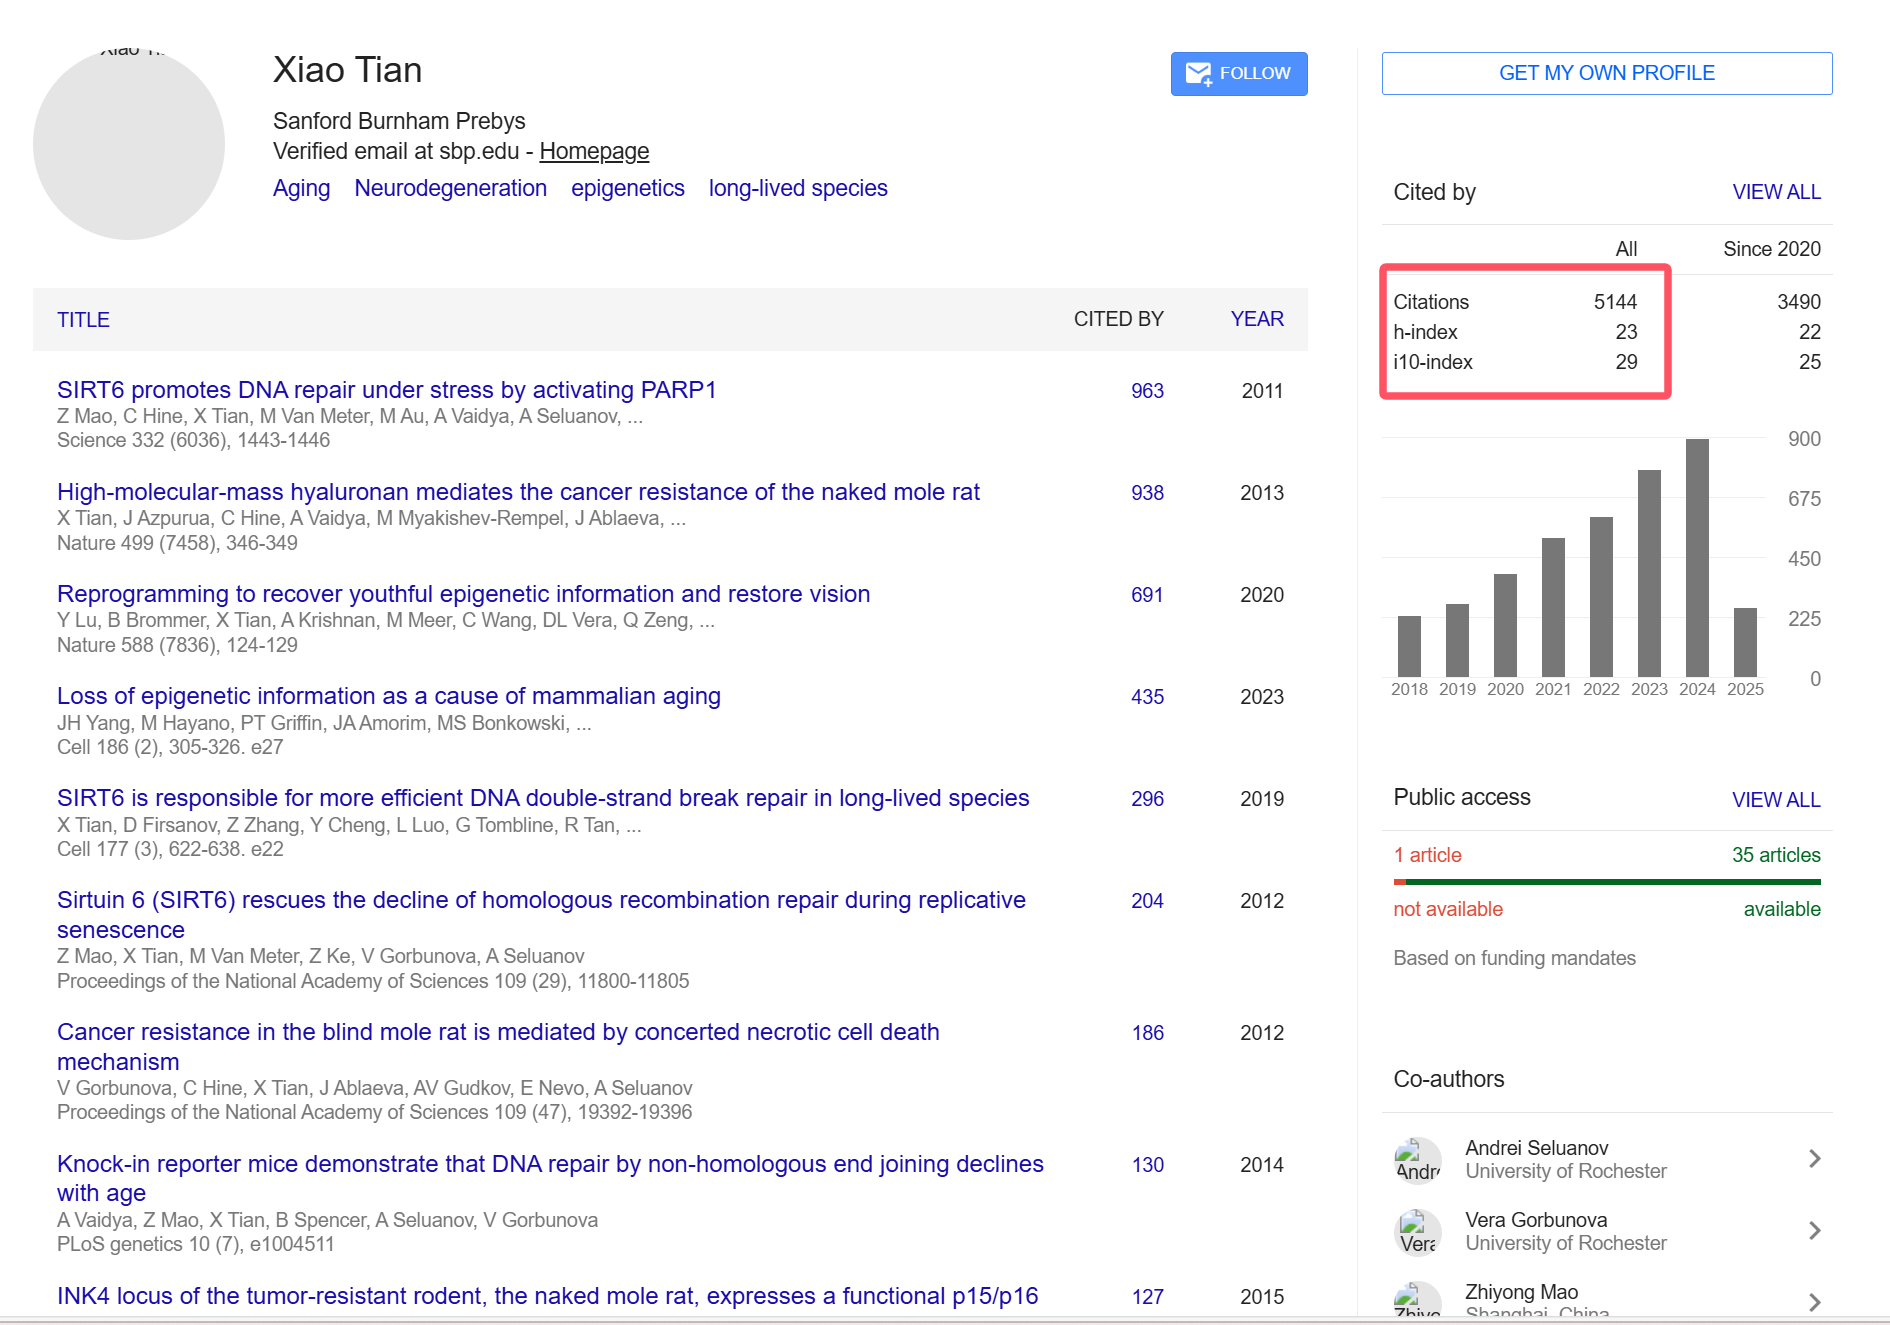
\includegraphics[width=0.4\textwidth]{image/第0章/google_scholar_XiaoTian.png}
    \hfill
    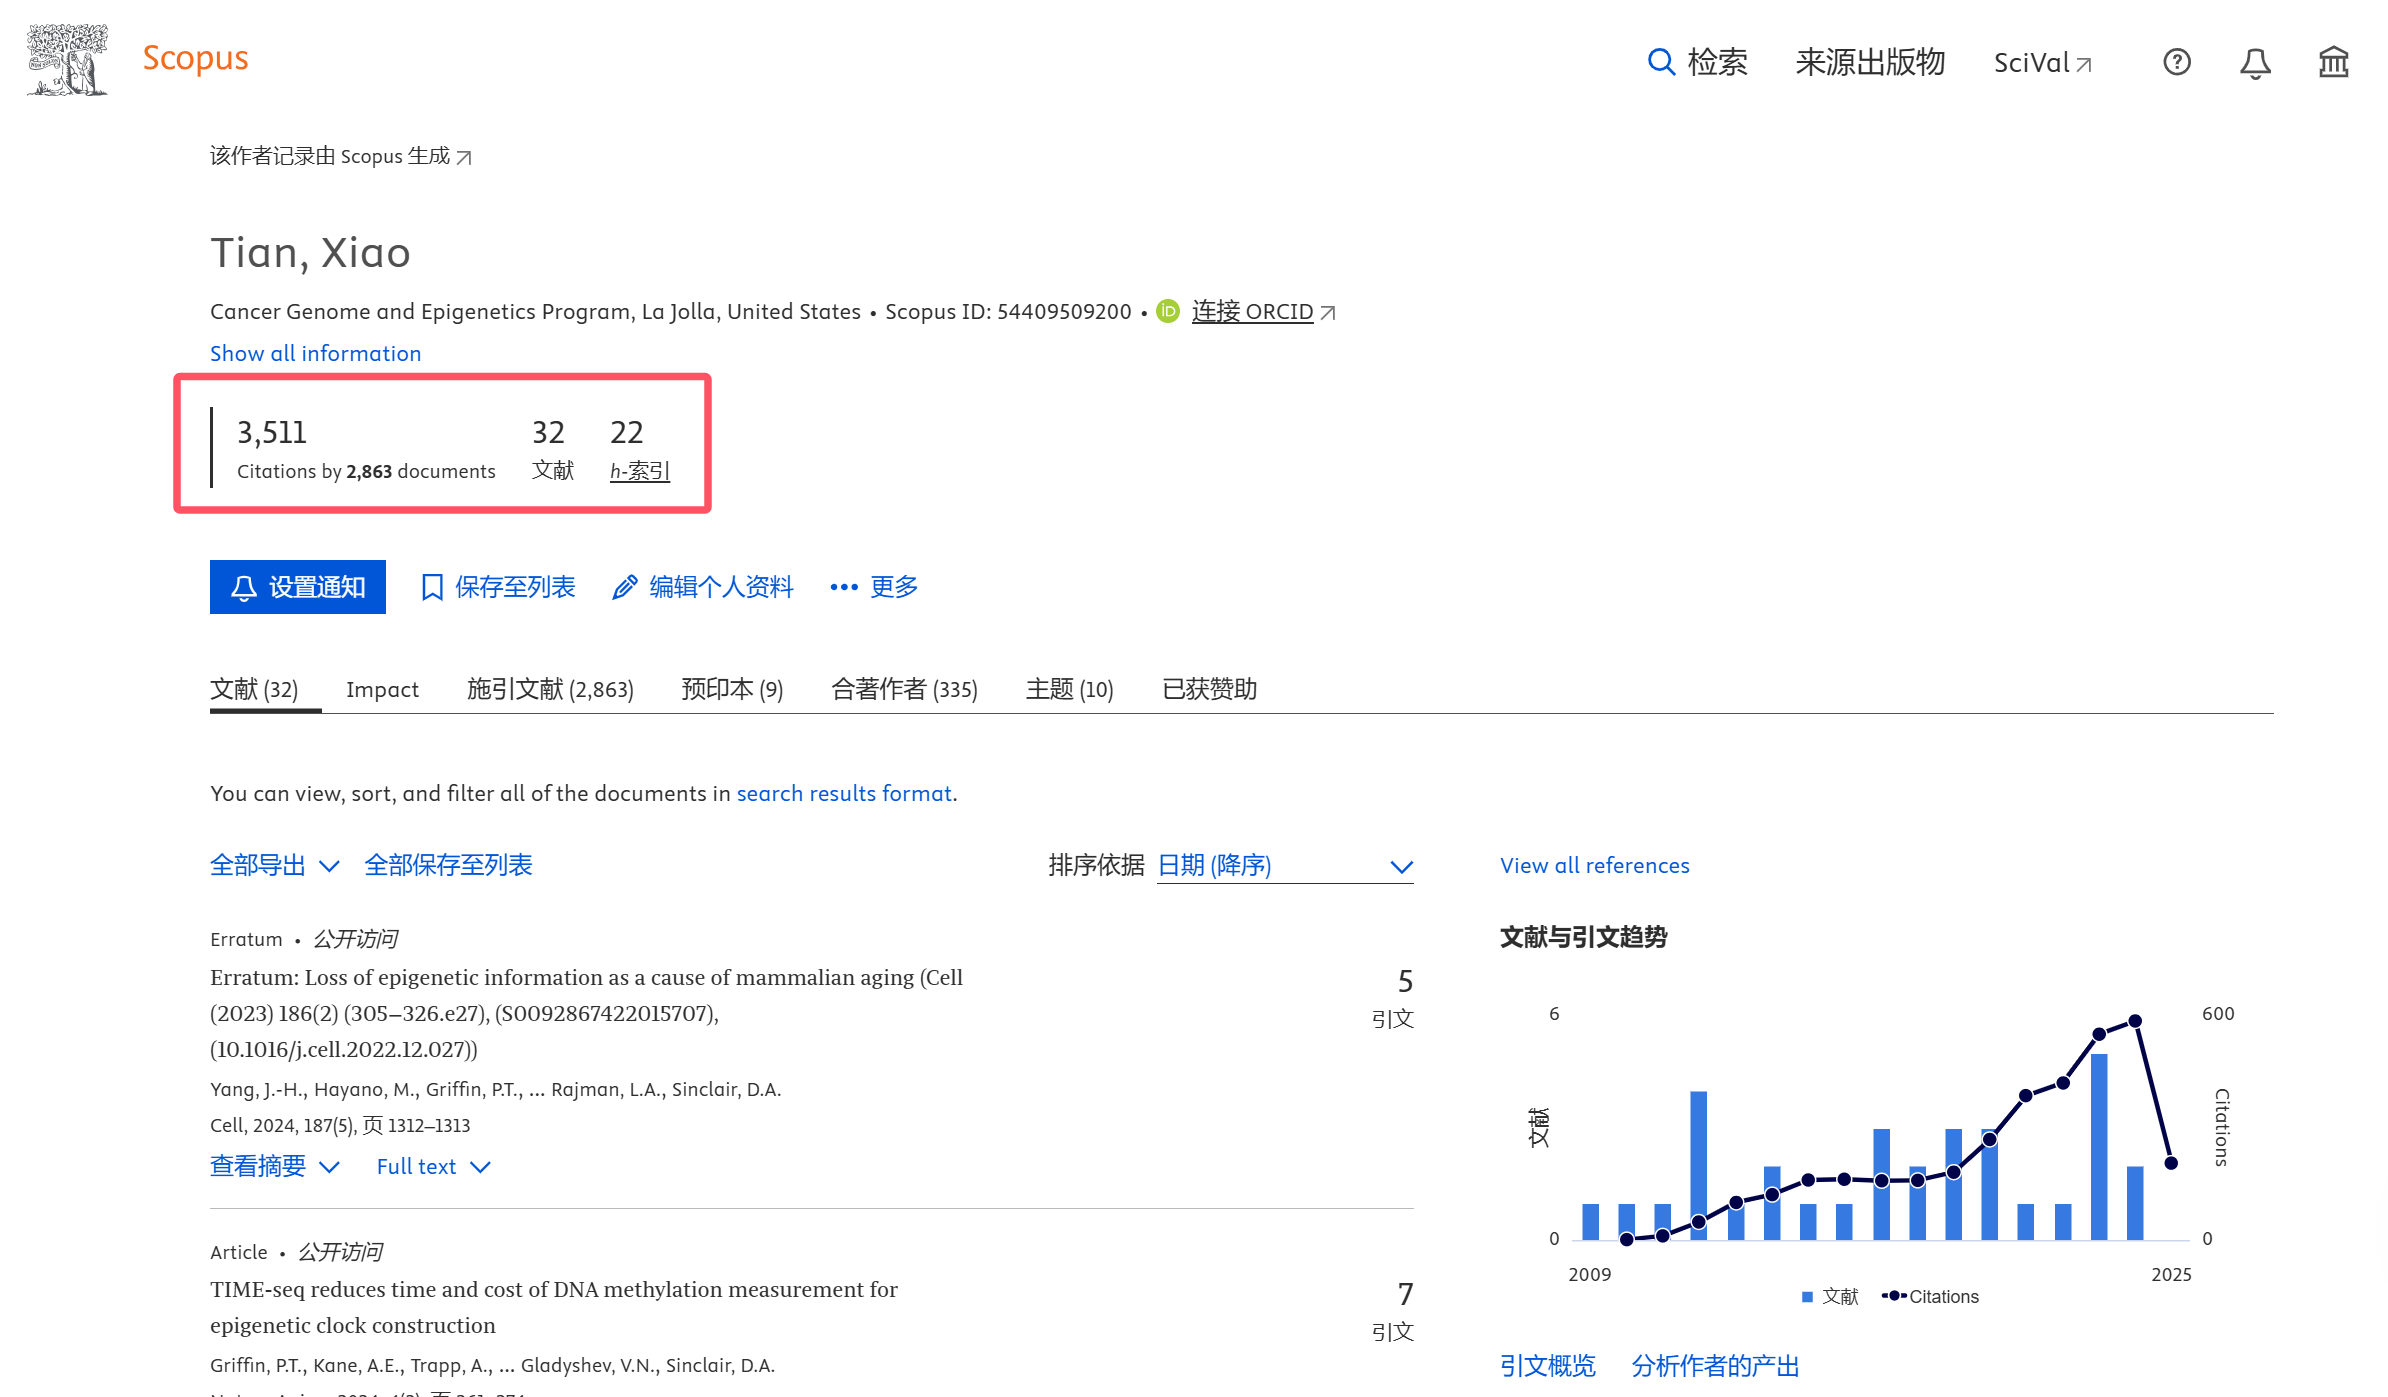
\includegraphics[width=0.45\textwidth]{image/第0章/Scopus_XiaoTian.png}
    \caption{Google scholar以及Scopus查找引用}
\end{figure}

一般套瓷流程主要是按照大学进行查找，在大学网站中查找到心仪导师后再通过上述方法精确查找。不过通常情况下大学网站弯弯绕绕而且容易遗漏，不同大学也很不一样，比较费时费力。但是本次套瓷之后，Ph.D就轻松很多了，不要偷懒哦，不然到时候还是会去补课的。

也可以使用Google Scholar进行查找，不过按照机构作为关键词并指定profile时往往不全面。

也有一些网站资源可以查找导师，例如Aminder，academic tree，支持按照机构、主题或者按照学术关系进行查找。不过网站资源需要仔细甄别哦。

\begin{figure}[H]
    \centering
    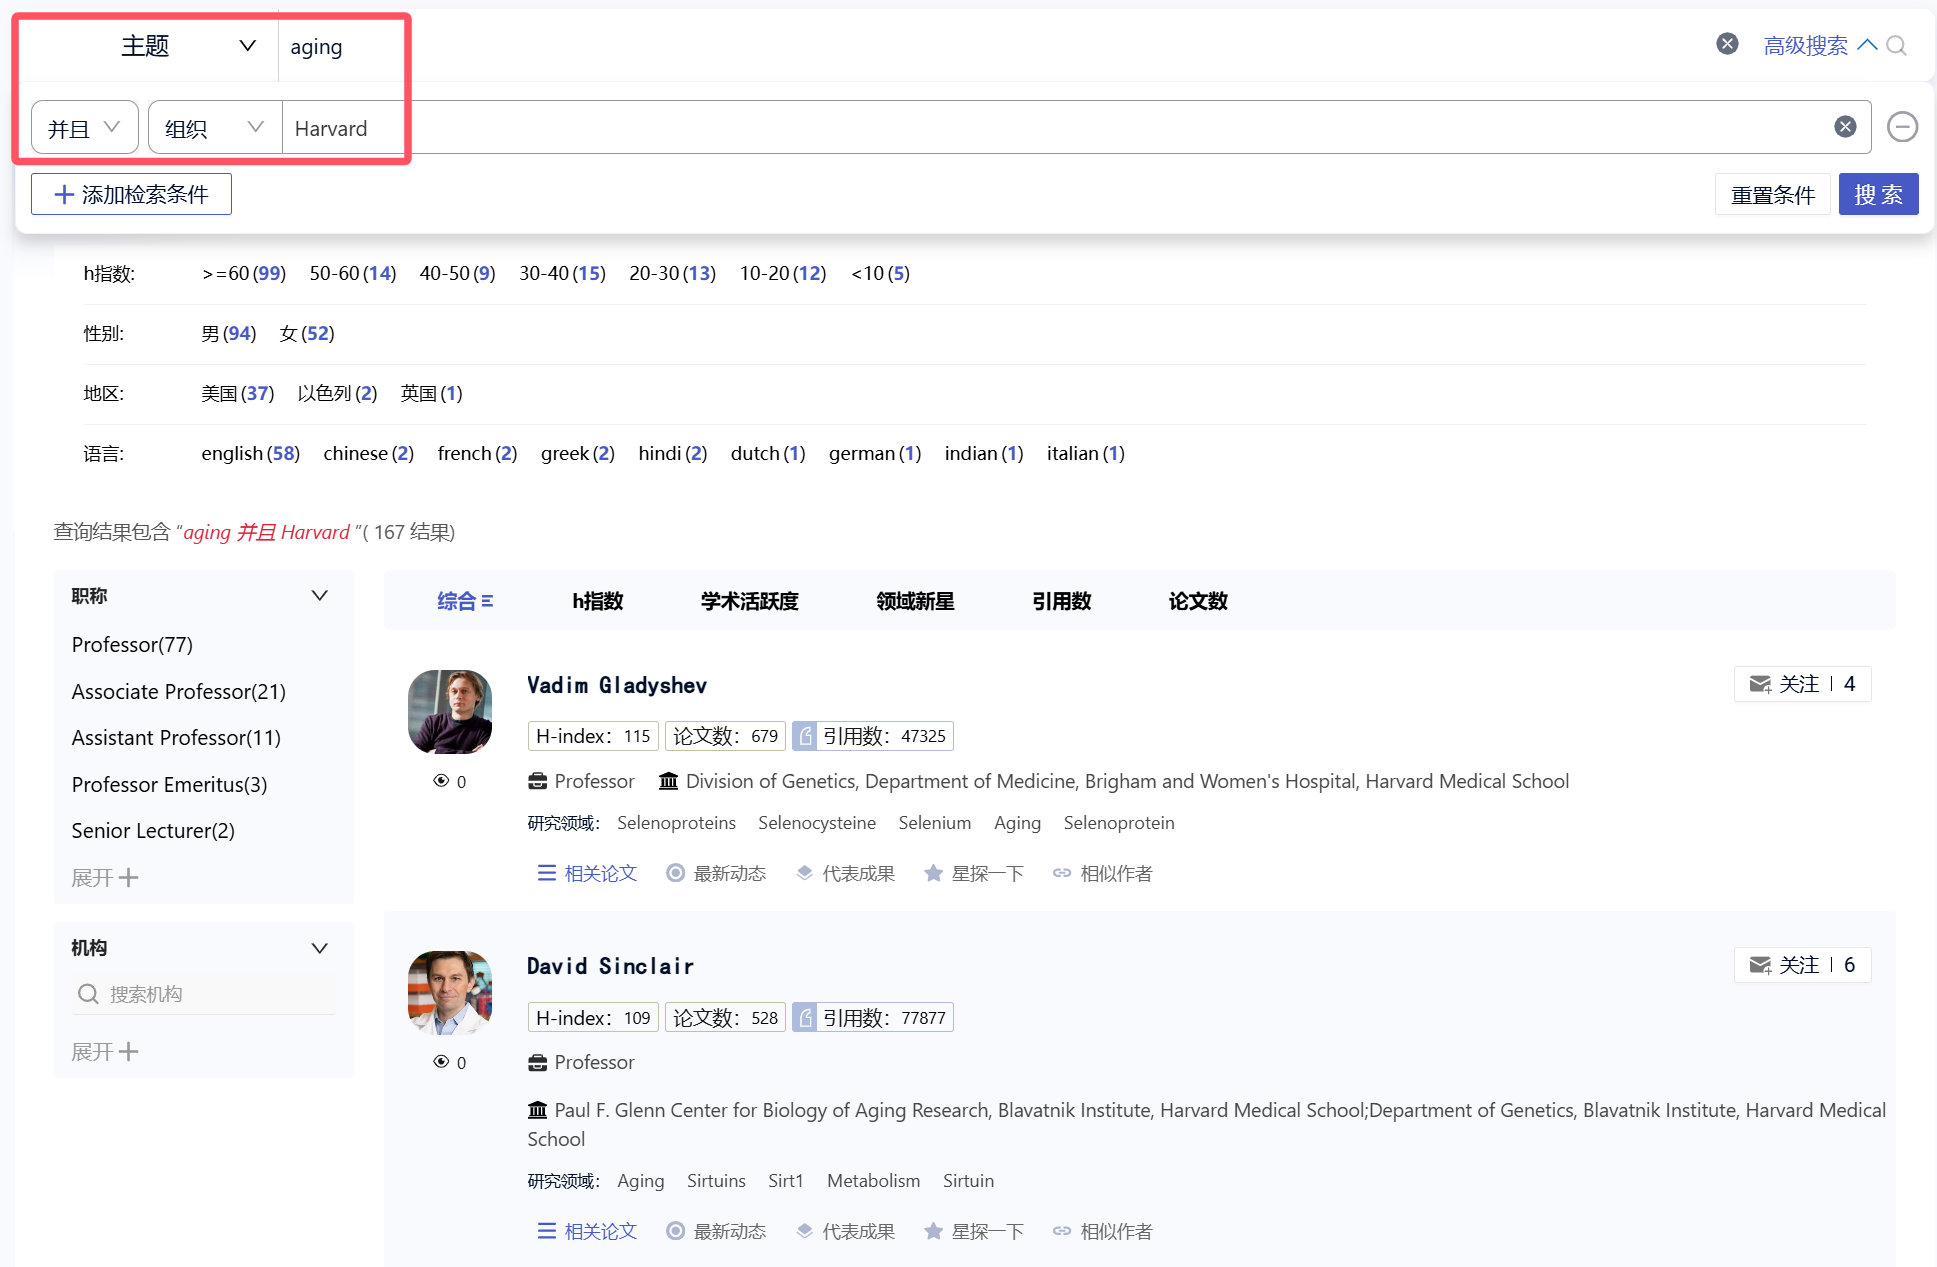
\includegraphics[width=0.5\linewidth]{image/第0章/Aminder.png}
    \caption{Aminder使用界面}
\end{figure}

\begin{figure}[H]
    \centering
    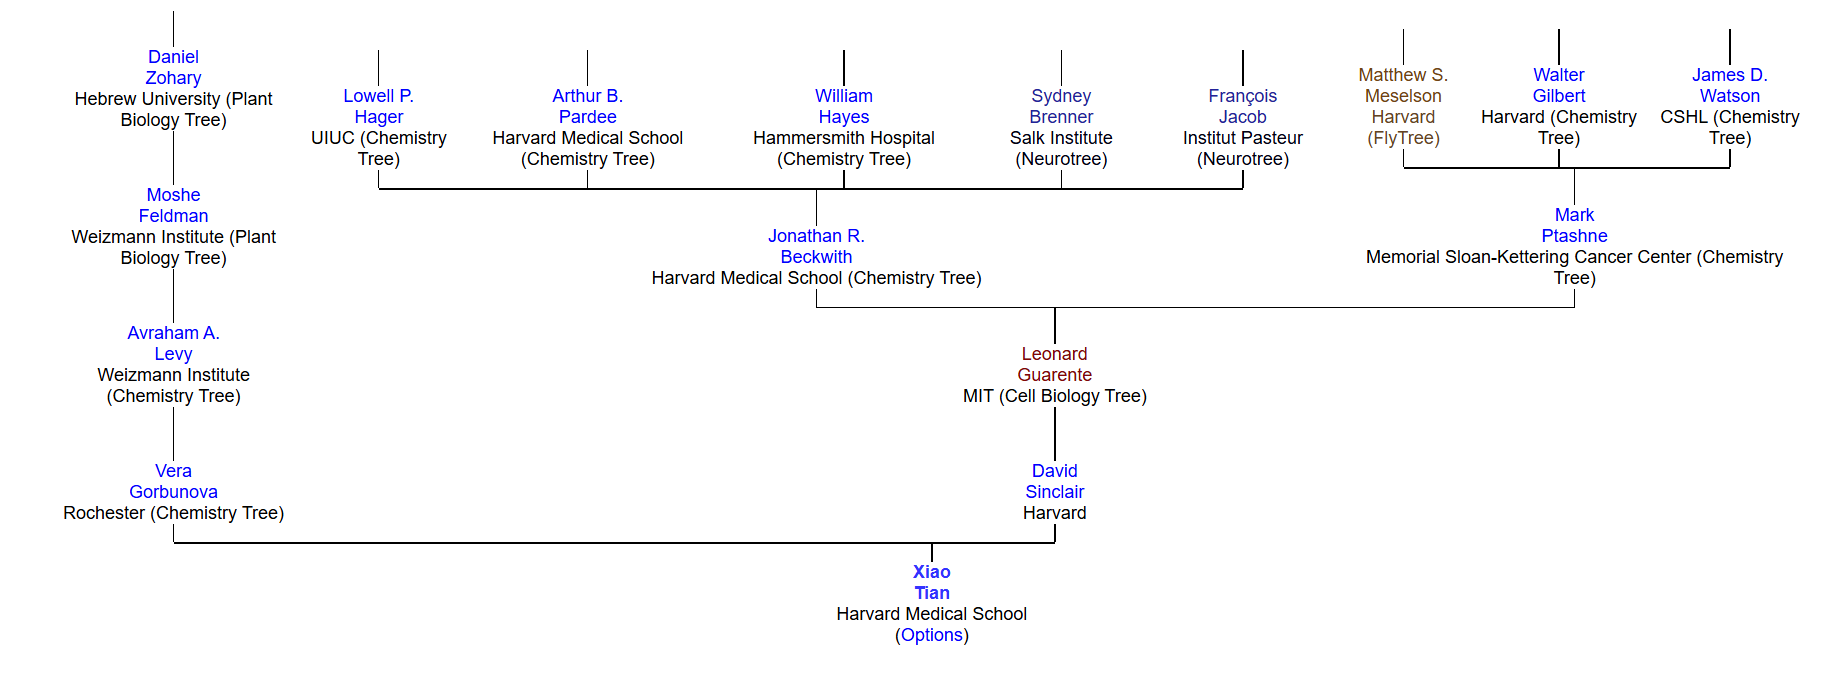
\includegraphics[width=0.8\linewidth]{image/第0章/aca-tree.png}
    \caption{academic tree使用}
\end{figure}

在academic tree可以直接查看导师的学术关系。例如Xiao Tian在罗彻斯特做博士和博后的导师Vera Gorbunova以及Xiao之后在Harvard的博后导师Sinclair。这有助于了解目标导师的合作网络和学术背景。

\section*{导师评价}

评价一个导师之前，请允许我介绍一些概念：

\begin{itemize}
    \item 影响因子（Impact factor/IF）指某一期刊的文章在特定年份或时期被引用的频率，是衡量学术期刊影响力的一个重要指标。计算方法：某期刊前两年总被引次数除以其前两年总发文量。
    \item 被引次数（Citations）是一篇文章被引用的次数。影响因子是针对于期刊而言的，被引次数则是针对单一一篇论文而言的，有区别。
    \item H指数（H index）是一个混合量化指标，可用于评估研究人员的学术产出数量与学术产出水平。

    H-index的计算方法略显复杂。以下引子wikipedia：“赫希认为：一个人在其所有学术文章中有N篇论文至少被引用了至少N次，他的H指数就是最大的这个N。如美国耶鲁大学免疫学家理查德·弗来沃发表的900篇文章中，从低到高，符合107篇被引用了107次以上，但是不符合108篇分别被引用至少108次的条件，他的H指数是107。
\end{itemize}

评价一名科研工作者的科研能力，最常用的就是引用量以及H-index等指标；课题组情况；经费情况……

\subsection*{科研能力}

对于引用以及文章\footnote{摘自金腾川老师的PPT}：

首先，论文被引用次数很重要， PI教授>1000，国内外要求差不多；H-index也是很重要的参考标准 (所有署名论文） PI教授>10 ， 国内外要求差不多；国内一流大学中科院研究所（前20名），正教授（研究员） 要求和美国普通大学（AP） 差不多： 有至少一篇CNS主刊（20分以上） ， 加10分以上两篇， 加5分以上5篇。 一区5篇。 

当然，该评价过程需要考虑到领域等问题。例如热门的免疫以及肿瘤等领域，引用量相对比较大。

查找引用量以及H-index可以使用Google Scholar（校园网现在可以直接连接，不需要翻墙）或者scopus等，由于收录计算引用方式不同，不同平台搜索略有不同。

\subsection*{funding}
评价以及选择导师的一个重要指标就是funding。对于近期国外的情况，更需要参考国外导师的funding情况。需要注意的是funding资助的常规周期为3-5年，如果funding在某年过后大幅缩减，很可能offer逐渐缩减直至平衡。
招收一个博士生最低的成本是30W刀左右（工资一年4W左右）

过去由于美国科研基金的重要来源是NIH，可以在\href{https://reporter.nih.gov}{NIH RePORTER}查询NIH funding进而推测导师的整体funding情况。

\begin{figure}[H]
    \centering
    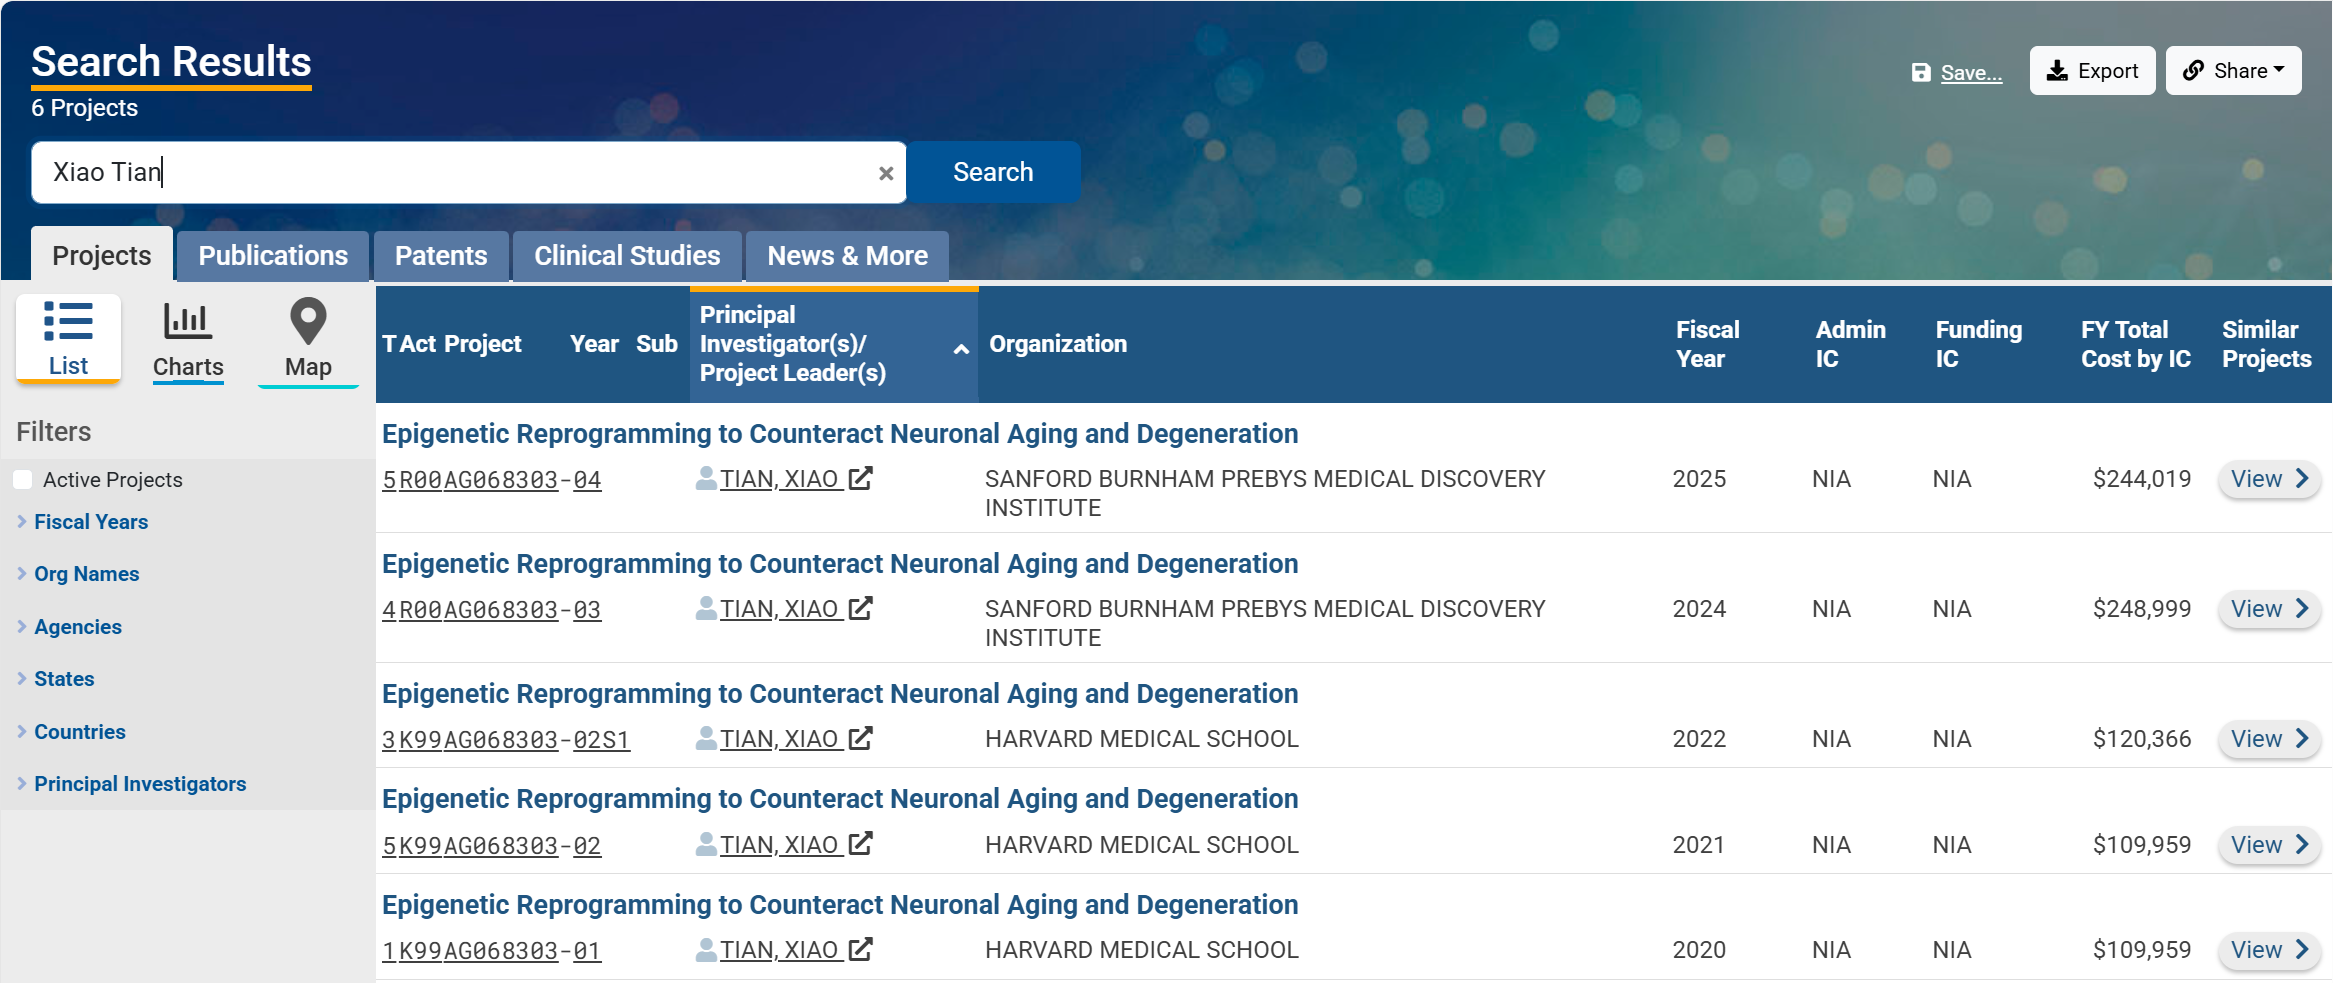
\includegraphics[width=0.7\linewidth]{image/第0章/NIH-funding-Xiao.png}
    \caption{NIH funding of Xiao Tian}
\end{figure}

\begin{figure}[H]
    \centering
    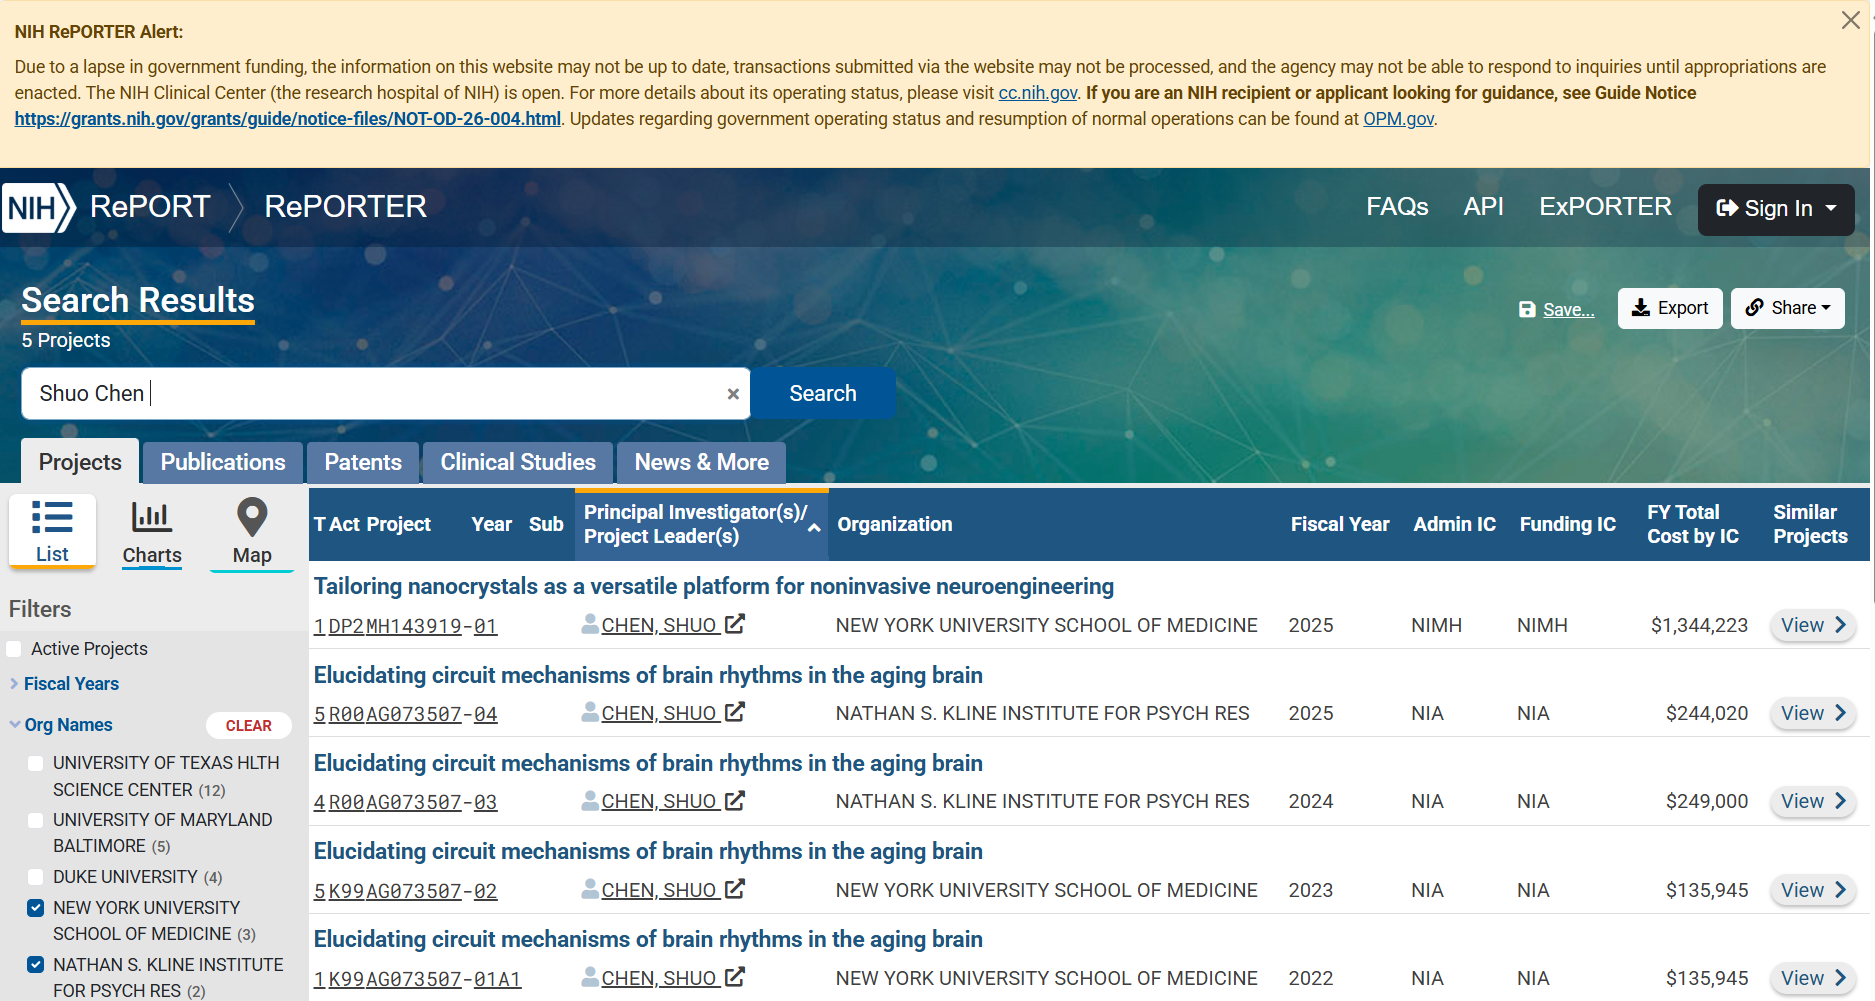
\includegraphics[width=0.7\linewidth]{image/第0章/NIH-funding-Shuo.png.png}
    \caption{NIH funding of Shuo Chen}
\end{figure}
以上图为例，NIH的K99/R00 funding是专门为博士后研究人员设计的过渡型资助，帮助他们从“导师指导下的博士后阶段”平稳过渡到“独立PI（助理教授）”阶段。R01是导师作为独立PI申请的基金，代表导师拥有独立申请的能力。Shuo目前已经有了DP开头的funding（类似R01），funding情况较好；Xiao目前还未申请到独立PI的基金。

\subsection*{管理方式}
某天在科大电梯里听两位导师“吐槽”：现在的信息渠道多了，学生都变聪明了，很难PUA。科大尚且如此，其他地方可见一斑。

良好的科研环境下，导师应当把学生视为处于训练中的合作者，而不是可随意替换的消耗品。这种“尊重”并不等于放任，也不等于降低要求；它更多体现在边界清晰、沟通透明、反馈及时、对学生的职业发展负责。因此，在你后续选择导师与课题组时，除了看论文与经费，更要学会识别：这个组是否真的理解并尊重不同 career stage 的训练逻辑——这往往比单纯的“名气”更能决定你未来几年是高质量成长，还是高强度消耗。

\begin{enumerate}
    \item 课题组人员组成：如果课题组成员来源比较多样化（例如包含一部分亚洲人），该实验室往往国际化程度较高，存在歧视的可能性更小。
    \item 课题组大小：一般导师一年往往只招收1-2Ph.D，2个左右的MSs，才会有足够的精力和课题组每个学生有充足的交流。如果课题组过大，往往会分给小老板或者博后负责，这时候你的体验感就取决于小老板了。
    \item 管理方式：是否需要打卡等……
\end{enumerate}

导师评价可以查找一些网站，例如：研控\href{https://www.yankong.org/}{yankong.org}。但是请注意，网站评价往往是片面的，可能会有恶意评论。可作为参考，但是一定要结合实际情况。

%20260202-ez